\documentclass[margin,line]{res}

\oddsidemargin -.5in
\evensidemargin -.5in
\textwidth=6.0in
\itemsep=0in
\parsep=0in

\newenvironment{list1}{
  \begin{list}{\ding{113}}{
      \setlength{\itemsep}{0in}
      \setlength{\parsep}{0in} \setlength{\parskip}{0in}
      \setlength{\topsep}{0in} \setlength{\partopsep}{0in}
      \setlength{\leftmargin}{0.17in}}}{\end{list}}
\newenvironment{list2}{
  \begin{list}{$\bullet$}{
      \setlength{\itemsep}{0in}
      \setlength{\parsep}{0in} \setlength{\parskip}{0in}
      \setlength{\topsep}{0in} \setlength{\partopsep}{0in}
      \setlength{\leftmargin}{0.2in}}}{\end{list}}
%\usepackage{graphicx}



\begin{document}

\begin{figure}
\vspace{-2cm}

\hfill
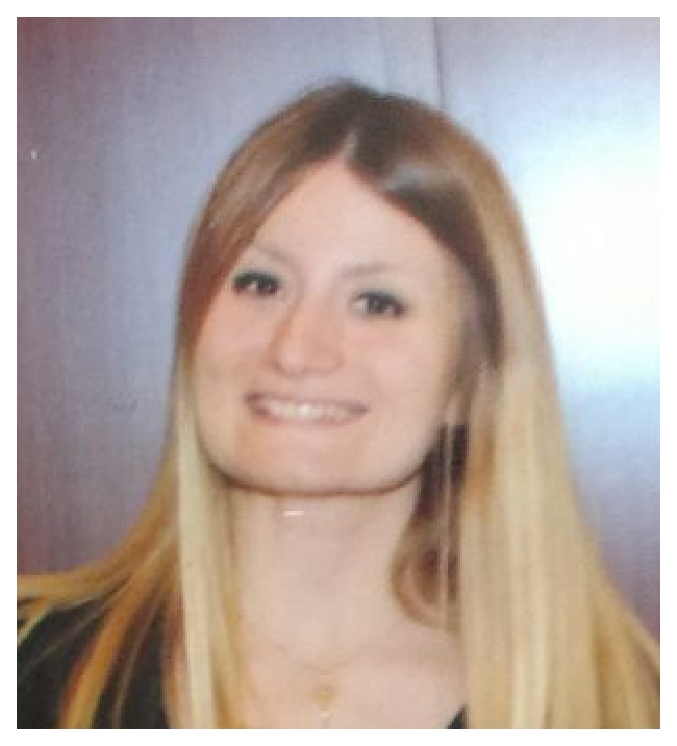
\includegraphics[scale=0.31]{elguz.eps}

\vspace{-1cm}

\end{figure}

\name{Elgiz Baskaya \vspace*{.1in}}

\begin{resume}
\section{\sc Contact Information}
\vspace{.05in}
\begin{tabular}{@{}p{3in}p{3in}}
7, avenue Edouard Belin CS 54005 & {\it Mobile:}  (+33)616460022 \\
31055 Toulouse Cedex 4 France     & {\it E-mail:}  benelgiz@gmail.com\\
\end{tabular}


\section{\sc Research Interests} Fault Detection and Diagnosis, Machine Learning, Fault Tolerant Control, Estimation and Control

\section{\sc Education}

{\bf PhD., Ecole Doctoral Aeronautique Astronautique} \hfill {\bf  2016 - Present (2018 Expected)}\\
\vspace*{-.05in}
\begin{list1}
\item[] Universite Paul Sebatier, Toulouse, France
\begin{list2}
\vspace*{.05in}
\item Dissertation Topic:  ``Fault Tolerant Control of Remotely Piloted Aircraft Systems"
%\item Advisor:  Prof. Dr. Ibrahim Ozkol
%\item GPA: /4.00
\end{list2}
\end{list1}

{\bf PhD., Interdisciplinary Aeronautical and Astronautical Sciences} \hfill {\bf  2010 - Present (2017 Expected)}\\
{\em Faculty of Aeronautics and Astronautics}
\vspace*{.1in}
\begin{list1}
\item[] Istanbul Technical University, Istanbul, Turkey
\begin{list2}
\vspace*{.05in}
\item Dissertation Topic:  ``Heat Transfer Enhancement by Using Magnetic Nanofluids"
%\item Advisor:  Prof. Dr. Ibrahim Ozkol
%\item GPA: /4.00
\end{list2}
\end{list1}

{\bf M.Sc., Interdisciplinary Aeronautical and Astronautical Sciences}  \hfill {\bf  2007 - 2010}\\
{\em Faculty of Aeronautics and Astronautics}
\vspace*{.1in}
\begin{list1}
\item[] Istanbul Technical University, Istanbul, Turkey
\begin{list2}
\vspace*{.05in}
\item Thesis:  ``Sensor Fusion Based Attitude Determination for Small Satellites''
%\item Dissertation Topic:  ``Hierarchical Models for Multiple Ratings
 %in Performance-Based\\ \hspace*{1.23in} Student Assessments.''
%\item Advisor:  Prof. Chingiz Hajiyev
%\item GPA: 3.91/4.00
\end{list2}
\end{list1}

{\bf B.S., Aerospace Engineering}\hfill {\bf 2002 - 2007}\\
{\em Faculty of Aeronautics and Astronautics}
\vspace*{.1in}
\begin{list1}
\item[] Istanbul Technical University, Istanbul, Turkey 
\begin{list2}
\vspace*{.05in}
\item Graduation Project: ``Transfers Between Satellites and Planets Through Trajectories \\ \hspace*{1.23in} on Stability Boundary'' 
%\item Advisor:  Prof. Umur Daybelge
\end{list2}
\end{list1}


%\section{\sc Honors and Awards}
%\begin{list1}
%\item[]
%\begin{list2}
%\vspace*{.05in}
%\item Listed in Marquis Who's Who in the World 2010\\
%\item High Honor Student in each semester with GPA: $3.91/4.00$ (Ph.D.)\\
%\item Best Academic Work in ``Mobil Gelecek'' competition by Turkcell (leading telecommunications operator of Turkey), 2007\\
%\item National Science Foundation (TUBITAK) Graduate Research Fellowship, 2005\\
%\item Honored with Dean's Award upon graduation\\
%\item Ranked $2^{nd}$ in department, $5^{th}$ in college with GPA: $3.72/4.00$ (B.S.)\\
%\item Vehbi Koc Scholar Award (SPA$>3.50$) in each semester (B.S.)\\
%\end{list2}
%\end{list1}
%NSF Vertical Integration of Research and Education in Statistics and
%Mathematical Sciences\\ (VIGRE) teaching fellowship.
%
%
\section{\sc Academic Experience}

{\bf Researcher - The ENGIE Ineo - Grope ADP - SAFRAN RPAS Chair} \hfill {\bf 2015 - Present}\\
{\em Ecole National l'Aviation Civile}, Toulouse, France \\
Designing fault diagnosis algorithms using machine learning techniques to enable a safe integration of drones into airspace. Algorithms designed will be a part of Paparazzi open-source autopilot system and be tested in real flights held under lab URI-DRONES of civile aviation institute of France, ENAC.

{\bf Research Assistant - Faculty of Aeronautics \& Astronautics} \hfill {\bf 2009 - 2015}\\
{\em Istanbul Technical University}, Istanbul, Turkey

{\bf Researcher - TUBITAK 113E595 }\hfill {\bf 2014 - 2015}\\
{\em Development of methods and algorithms for the integrated attitude
determination systems with in-flight sensor calibration, long-term 
planning guidance and fault-tolerant attitude control for the small 
information satellites, }  \\
Worked on robust attitude determination algorithms, Earth's Magnetic Field modeling, orbit propagation. This is a joint project with Samara State Technical University under the guidance of Prof. Chingiz Hajiyev and Yevgeny Somov. The project is funded by TUBITAK and Russian Science Foundation.
\vspace*{-.05in}

%{\bf Researcher - TUBITAK 113E595 }\hfill {\bf 2013}\\
%{\em Investigation of MHD systems effectiveness during re-entry (submitted) \\
%Undersecretariat for Defence Industries}  \\
%Investigation of the possibilities MHD systems offer for enhancement of the heating problems and deceleration issues a re-entry vehicle should survive, specifically for low density atmosphere cases.
%\vspace*{-.05in}

{\bf Researcher - Control and Avionics Laboratory}\hfill {\bf 2012 - 2014}\\ 
{\em High precision ADCS and indiginous bus architecture design and development project for Nano Satellites, TUBITAK 106M523}\\
Developed the onboard orbit propagator and attitude determination software in MATLAB for ITUpSAT 2, which is the  $2^{nd}$ small satellite project of ITU funded by TUBITAK. Additionally, worked on the design and development of the software/hardware-in-the loop system utilizing MATLAB/ 
Simulink and STKConnect Module to verify the indigenous ADCS which enjoys a redundant reaction wheel set for reliability.
\vspace*{-.05in}

{\em Resillience2050, EU 7th RTD Framework Programme }  \\
Worked on Decision Support Tools for Air Traffic Management to enable designs fostering safety, agility and resillience for Air Traffic Management under the guidance of Asc. Prof. Gokhan Inalhan. 
\vspace*{-.2in}

{\em Real time ATC Operator and Pilot Automation and Decision - Support Systems Design for New ATM Concept, TUBITAK 111M167 }  \\
Worked on Decision Support Tools for Air Traffic Management. Specialized on development of algorithms to estimate trajectory of aircraft and detect collision in the presence of uncertainties under the guidance of Asc. Prof. Gokhan Inalhan. The project is funded by TUBITAK.
\vspace*{-.05in}

{\bf Researcher - Space Systems Laboratory}\hfill {\bf 2008 - 2010}\\ 
{\em Pico Satellite Design, Development of Engineering and Flight Models, TUBITAK 106M082 }\\ 
System Engineer during the design, assembly and test phases of ITUpSAT 1, which was launched on 23 September 2009 from Satish Dhawan Space Center India. ITUpSAT 1, headed by Prof. Dr. Rustem Aslan and funded by TUBITAK, is the first orbiting satellite made in Turkey.
\vspace*{-.05in}

{\bf Researcher - Vestel Defense Industry} \hfill {\bf Fall 2008}\\
Studied on verification of the estimated model parameters with the use of measurements via least squares method under the guidance of Prof. Chingiz Hajiyev.
\vspace*{-.05in}

{\bf Researcher - Vestel Defense Industry} \hfill {\bf Spring 2007}\\
Developed codes on estimation of aircraft model using Extended Kalman Filter under the guidance of Prof. Chingiz Hajiyev.
\vspace*{-.05in}

\section{\sc Teaching Experience}

{\bf Teaching Assistant - Faculty of Aeronautics \& Astronautics}  \hfill {\bf 2009 - 2015}\\
{\em Istanbul Technical University, Istanbul, Turkey}
\vspace*{-.05in}

Probability  \& Statistics  \hfill {Spring 2015, Spring 2014}\\
Orbital Mechanics  \hfill {Spring 2014}\\
Heat Transfer \hfill {Fall 2013}\\
Thermodynamics \hfill {Spring 2013}\\
Attitude Determination  \& Control  \hfill {Fall 2014, Fall 2013, Fall 2012, Fall 2011}\\
Avionics \hfill {Spring 2012, Fall 2011}\\
Principles of Aircraft Design \hfill {Spring 2012, Fall 2011}\\
Flight Stability and Control, \hfill {Fall 2011}\\
Automatic Control \hfill {Spring 2011, Spring 2009}\\
Introduction to Sci\&Eng. Comp. -  C Programming Language \hfill {Spring 2011}\\
Dynamics \hfill {Fall 2009}\\
Spacecraft System Design \hfill {Spring 2009}\\
\vspace*{-.20in}

Presented \textquotedblleft  \emph{Developments in Satellite Technology in Turkey}\textquotedblright\, during GAP Astronomy Journey to Southeastern Anatolia to educate and inform students on recent subjects. Funded by Republic of Turkey, Regional Development Administration, \\Southeastern Anatolia\hfill {October 11 - 22, 2010}
\vspace*{-.05in}

Course given to Okyanus College students on  \textquotedblleft  \emph{Space, Science and Technology Demonstrations}\textquotedblright\, Okyanus College, Istanbul\hfill {Fall 2009, Spring 2010}
\vspace*{-.05in}

\section{\sc Internship}

{\bf Baykar Technologies}, Istanbul, Turkey\\
{\em Intern} \hfill {\bf Summer 2006}\\
Summer Internship in one of the two unmanned air vehicle design companies in Turkey. Trained on Kalman Filtering.

{\bf TAI (Turkish Aerospace Industries, Inc.)}, Ankara, Turkey\\
{\em Intern} \hfill {\bf Summer 2005}\\
Summer Internship in R\&D Department.
Trained on satellite thermal control system. Developed codes on thermal network method in Matlab to verify the in-house developed satellite thermal system simulator.

\section{\sc Publications}

Baskaya, E., Bronz, M., Delahaye, D. \textquotedblleft Fault Detection \& Diagnosis for Small UAVs via Machine Learning \textquotedblright\  \emph{ $36^{th}$ IEEE/AIAA Digital Avionics Systems Conference (DASC),} September 17 - 21, 2017 (accepted)

Baskaya, E., Bronz, M., Delahaye, D. \textquotedblleft Flight Simulation of a MAKO UAV for Use in Data-Driven Fault Diagnosis \textquotedblright\  \emph{  $9^{th}$ International Micro Air Vehicles,} September 18 - 21, 2017 (submitted)

Baskaya, E., Manfredi, G., Bronz, M., Delahaye, D. \textquotedblleft Flexible open architecture for UASs integration into the airspace: Paparazzi autopilot system\textquotedblright\  \emph{ $35^{th}$ IEEE/AIAA Digital Avionics Systems Conference (DASC),} September 25 - 29, 2016

E. Baskaya, G. Komurgoz, I. Ozkol, \textquotedblleft A bioinspired impedence pump in the presence of magnetic nanofluids, \textquotedblright\ (in preperation)

E. Baskaya, G. Komurgoz, I. Ozkol, \textquotedblleft Investigation of Oriented Magnetic Field Effects on Entropy Generation in an Inclined Channel Filled with Ferrofluids, \textquotedblright\ (submitted)

E. Baskaya, G. Komurgoz, I. Ozkol, \textquotedblleft Entropy Generation and Equipartition Phenomenon Investigation in a Variable Viscosity Channel Flow under Constant Magnetic Field via Generalized Differential Quadrature Method (GDQM) , \textquotedblright\ \emph{Heat and Mass Transfer, Springer,} (submitted)

E. Baskaya, G. Komurgoz, I. Ozkol, \textquotedblleft Analysis of Variable Viscosity Channel Flow under Constant Magnetic Field via Generalized Differential Quadrature Method, \textquotedblright\ \emph{Advanced Materials Research,} vol. 1016, pp.564-568, 2014

E. Baskaya, U. Daybelge, A. Sofyali, E. Topal, C. Yarim, \textquotedblleft Developments in Astrodynamics in the Light of Chaos \textquotedblright\ \emph{Journal of Istanbul Kultur University,} vol.4, pp.191-212, 2006

E. Baskaya, G. Komurgoz, I. Ozkol \textquotedblleft Analysis of a Variable Viscosity Channel Flow under Constant Magnetic Field via Generalized Differential Quadrature Method\textquotedblright\ \emph{ ICMAE $5^{th}$ International Conference on Mechanical and Aerospace Engineering}, July 18 - 19, 2014 

E. Baskaya, M. Fidanoglu, et at. \textquotedblleft Investigation of MHD Natural Convection Flow Exposed to a Variable Magnetic Field via Differential Quadrature Method\textquotedblright\ \emph{ ASME $12^{th}$ Biennial Conference on Engineering Systems Design and Analysis}, June 24 - 27, 2014 

M. Fidanoglu, E. Baskaya, et at. \textquotedblleft Application of Differential Quadrature Method and Evolutionary Algorithm to MHD Fully Developed Flow of a Couple-Stress Fluid in a Vertical Channel With Viscous Dissipation and Oscillating Wall Temperature\textquotedblright\ \emph{ ASME $12^{th}$ Biennial Conference on Engineering Systems Design and Analysis}, June 24 - 27, 2014 

Elgiz Baskaya, G. Inalhan, et al. \textquotedblleft Design and Development of a Reliable ADCS and Indigenous Bus Architecture for Nanosatellites : ITUpSAT II\textquotedblright\ \emph{$63^{rd}$ International Astronautical Congress}, October 1- 5, 2012

E. Baskaya, U. Eren, G. Inalhan \textquotedblleft Development of High - Precision Attitude Determination and Control  System : ITUpSAT II project \textquotedblright\ \emph{National Aeronautical and Astronautical Conference}, September 12 - 14, 2012

E. Baskaya, E. Koyuncu, G. Inalhan \textquotedblleft Design of a Multi - Purpose Nanosatellite Bus : ITUpSAT II project \textquotedblright\ \emph{National Aeronautical and Astronautical Conference}, September 12 - 14, 2012

E. Baskaya, U. Eren, et al. \textquotedblleft A Precise ADCS Design for ITUpSAT II\textquotedblright\ \emph{International Conference on Student Small Satellites}, April 25 - 27, 2012

U. Eren, E. Baskaya, et al. \textquotedblleft Design of a Flexible Bus System for ITUpSAT II\textquotedblright\ \emph{International Conference on Student Small Satellites}, April 25 - 27, 2012

E. Koyuncu, E. Baskaya, et al. \textquotedblleft ITUpSAT II : High - Precision Nanosatellite ADCS Development Project\textquotedblright\ \emph{ $5^{th}$ International Conference on Recent Advances in Space Technologies}, June 9 - 11, 2011

G. Inalhan, E. Koyuncu, E. Baskaya, et al. \textquotedblleft Design and Development of ITUpSAT II : On Orbit Demonstration of a High - Precision ADCS for Nanosatellites \textquotedblright\ \emph{ $8^{th}$ International ESA Conference on Guidance \& Navigation Control Systems}, June 5 - 10, 2011

E. Baskaya, C. Hajiyev, G. Inalhan \textquotedblleft Estimation of Small Satellite Attitude Dynamics via EKF using Magnetometers - ITUpSAT II Project\textquotedblright\ \emph{National Aeronautical and Astronautical Conference}, September 16 - 18, 2010
\vspace*{-.05in}

%\section{\sc Journal Papers}

%\newpage
\section{\sc Workshops}
E. Baskaya, \textquotedblleft ITUpSAT II ADCS : Getting Ready for Launch\textquotedblright\ \emph{ $8^{th}$ Annual CubeSat Developers' Workshop}, April 20 - 22, 2011
\vspace*{-.05in}


E. Baskaya, G. Inalhan \textquotedblleft ITUpSAT II - Nanosatellite Platform for In-Space R\&D\textquotedblright\ \emph{ $7^{th}$ Annual CubeSat Developers' Workshop}, April 21 - 23, 2010
\vspace*{-.05in}

\section{\sc Poster Presentations}

U. Eren, Elgiz Baskaya, et al. \textquotedblleft Design of a Flexible Nanosatellite Bus for Science Missions \textquotedblright\ \emph{AIAA SPACE 2012 Conference \& Exposition}, September 11- 13, 2012

Elgiz Baskaya, U.Eren, et al. \textquotedblleft ITUpSAT II - Design and Development \textquotedblright\ \emph{Innovation Week Turkey}, December 6- 8, 2012

\section{\sc Workshops, Meetings \& Lectures Attended }
Object Oriented Programming with C++, 160 hours course on Objected Oriented Programming  with C++ in C System Programmers Association, 2014 - 2015
\vspace*{-.05in}

C Programming Language Training and Certificate, 160 hours course on C Programming language in C System Programmers Association, 2013 - 2014
\vspace*{-.05in}

Practical Adaptive Control, International Graduate School on Control, by Prof Anuradha Annaswamy, MIT Active Adaptive Control Laboratory, May 15 - 19, 2017
\vspace*{-.05in}

Tutorial on Multi-Sensor Navigation Focus on UAV Navigation, by Assist. Prof. Demoz Gebre-Egziabher, University of Minnesota, November 14, 2016
\vspace*{-.05in}

Resillience 2050 Progress Meeting, November 15 - 16, 2012
\vspace*{-.05in}

Research in Decision Support Tools for Future Air Traffic Management, {\it HALA! SEZAR Research Network Summer School}, July 9 - 12 2012
\vspace*{-.05in}

Lecture on Space System Engineering \& CUBESATs by Prof. Dr. Eberhard GILL, May 24, 2012
\vspace*{-.05in}

Small Satellite Formations for Distributed Survelliance: System Design and Optimal Control Considerations, {\it NATO-RTO Lecture Series SCI-231}, April 14 - 15 2011
\vspace*{-.05in}

Multifunctional Structures and System Technologies for Small Spacecraft, {\it NATO RTO-AVT171}, April 12 - 15, 2010
\vspace*{-.05in}

Astronet Workshop, {\it The Astrodynamics Network}, March 30 - April 1, 2009 
%\begin{verbatim}http://www.nist.gov/speech/publications/tw00/html/abstract.htm#cp1-50\end{verbatim}

%\section{\sc Professional Experience}

%\section{\sc Reviewer}
%\begin{list2}
%\item ICC 2006
%\item Globecom 08
%\item Elsevier Signal Processing: Image Communications
%\item IEEE J-SAC Special Issue on Wireless Video Transmission
%\end{list2}

\section{\sc Skills}
\begin{list2}
\item Languages: Turkish (native), English (fluent)(Toefl IBT : 97), French(beginner)
\item Programming Languages : MATLAB, C, C++, Fortran
\item Simulation/ CAD Tools: MATLAB/Simulink, STK, STKConnect, Mathematica, R, CATIA
\item OS: MacOS, Linux, Windows
\end{list2}


\section{\sc Professional Activities}
\begin{list2}
\item	President of Aerospace Engineering Research Assistants in  Fall 2010 - Spring 2011
\item	Member of UUMK (Aeronautics and Astronautics Engineering Club)
\item	Member of TEGV (Turkish Education Volunteers)
\end{list2}


\section{\sc Recreational / Personal Activities}
\begin{list2}
\item	Pianist and Tango dancer in Galata Festival in 2007
\item	Pianist in AKM as PERA Fine Arts High-school students in 2000
\item	Licensed volleyball player in 1999 and 2000 and won two cups as the best team in the town
\item	Member of the best team in group discussion challenge throughout town in 2002
\end{list2}

%\section{\sc References}
%\begin{list2}
%\item Prof. Dr. Ibrahim Ozkol\\
%Istanbul Technical University, ozkol{@}itu.edu.tr
%\vspace*{.2in}
%\item {\bf Prof. Chingiz Hajiyev}\\ 
%Istanbul Technical University, Faculty of Aeronautics and Astronautics

%\begin{tabular}{@{}p{3in}p{3in}}
%Istanbul Teknik Universitesi   & {\it Mobile:}  (+90)506-512-28-51 \\
%Ucak ve Uzay Bilimleri Fakultesi	& {\it Work:} (+90)212-285-3105 \\
%Ayazaga Kampusu, Istanbul/Turkey 	& {\it E-mail:}  cingiz@itu.edu.tr\\
%\end{tabular}

%\vspace*{.2in}
%\item Asc. Dr. Guven Komurgoz\\
%Istanbul Technical University, komurgoz{@}itu.edu.tr
%\vspace*{.2in}
%\item Asc. Prof. Gokhan Inalhan\\
%Istanbul Technical University, inalhan{@}itu.edu.tr
%\vspace*{.2in}
%\item Prof. Umur Daybelge\\
%Istanbul Technical University, daybelge@itu.edu.tr
%\newpage
%\item {\bf Prof. Alim Rustem Aslan}\\
%Istanbul Technical University, Faculty of Aeronautics and Astronautics

%\begin{tabular}{@{}p{3in}p{3in}}
%Istanbul Teknik Universitesi   & {\it Mobile:}  (+90)532-480-34-49 \\
%Ucak ve Uzay Bilimleri Fakultesi	& {\it Work:}  (+90)212-285-7189/140 \\
%Ayazaga Kampusu, Istanbul/Turkey 	& {\it E-mail:}  aslanr@itu.edu.tr\\
%\end{tabular}



%\vspace*{.2in}
%\item Asc. Prof. Turgut Berat Karyot\\
%karyot@itu.edu.tr\\
%Istanbul Technical University
%\end{list2}


\end{resume}
\end{document} 